\documentclass[a4paper]{article}

\usepackage[spanish]{babel}
\usepackage{graphicx}
\usepackage{amsmath, amssymb}
\usepackage[margin=2cm]{geometry}
\usepackage{fancyhdr}
\usepackage{enumerate}
\usepackage[shortlabels]{enumitem}
\usepackage{parskip}
\usepackage[most]{tcolorbox}
\usepackage[hidelinks]{hyperref}
\usepackage{float}
\usepackage{setspace}
\usepackage{xspace}


\usepackage{tabularx}
\usepackage{ragged2e}
\newcolumntype{L}{>{\RaggedRight\arraybackslash}X}
\newcolumntype{C}{>{\Centering\arraybackslash}X}

% cabecera
\pagestyle{fancy}
\fancyhead[l]{Daniel Soto}
\fancyhead[c]{Problemas de Astronomía \#14}
\fancyhead[r]{\today}
\fancyfoot[c]{\thepage}
\renewcommand{\headrulewidth}{0.2pt} % linea horizontal

%% Definicion de comandos para formato de unidades fisicas %%
\newcommand{\m}{\text{m}}
\newcommand{\cm}{\text{cm}}
\newcommand{\mm}{\text{mm}}
\newcommand{\km}{\text{km}}
\newcommand{\s}{\text{s}}
\newcommand{\N}{\text{N}}
\newcommand{\g}{\text{g}}
\newcommand{\kg}{\text{kg}}
\newcommand{\Msolar}{\text{M}_\odot}
\newcommand{\Mterrestre}{\text{M}_\oplus}
\newcommand{\AU}{\text{AU}}
\newcommand{\ly}{\text{ly}}
\newcommand{\nT}{\text{nT}}
\newcommand{\keV}{\text{keV}}
\newcommand{\MeV}{\text{MeV}}
\newcommand{\GeV}{\text{GeV}}
\newcommand{\atoms}{\text{atoms}}
\newcommand{\K}{\text{K}}
\newcommand{\J}{\text{J}}
\newcommand{\particles}{\text{particles}}
\newcommand{\protones}{\text{p}^+}
\newcommand{\electrones}{\text{e}^-}
\newcommand{\Gy}{\text{Gy}}
\newcommand{\My}{\text{My}}
\newcommand{\nm}{\text{nm}}
\newcommand{\blank}{\rule{2cm}{0.4pt}\xspace}
\newcommand{\mol}{\text{mol}}
\newcommand{\W}{\text{W}}



\newcounter{problema}

\newtcolorbox[use counter=problema]{problema}[1][]{%
	breakable,
    colback=gray!15,
    colframe=gray!60,
    fonttitle=\bfseries,
    title={Problema~\theproblema:},
    boxrule=0.5mm,
    arc=3mm,
    boxsep=5pt,
    left=8pt,
    right=8pt,
    top=6pt,
    bottom=6pt,
    #1
}


\begin{document}

\begin{problema}

En 7 mil millones de años, nuestro sol se convertirá en una gigante roja, expulsando su atmósfera como una nebulosa planetaria y dejando atrás su núcleo denso. Este núcleo, de aproximadamente el tamaño de la Tierra, es lo que los astrónomos llaman una enana blanca y, al carecer de la capacidad de crear calor a través de reacciones nucleares, se enfriará de manera constante y se volverá más tenue como remanente estelar.
    
    \begin{figure}[H]
        \centering
        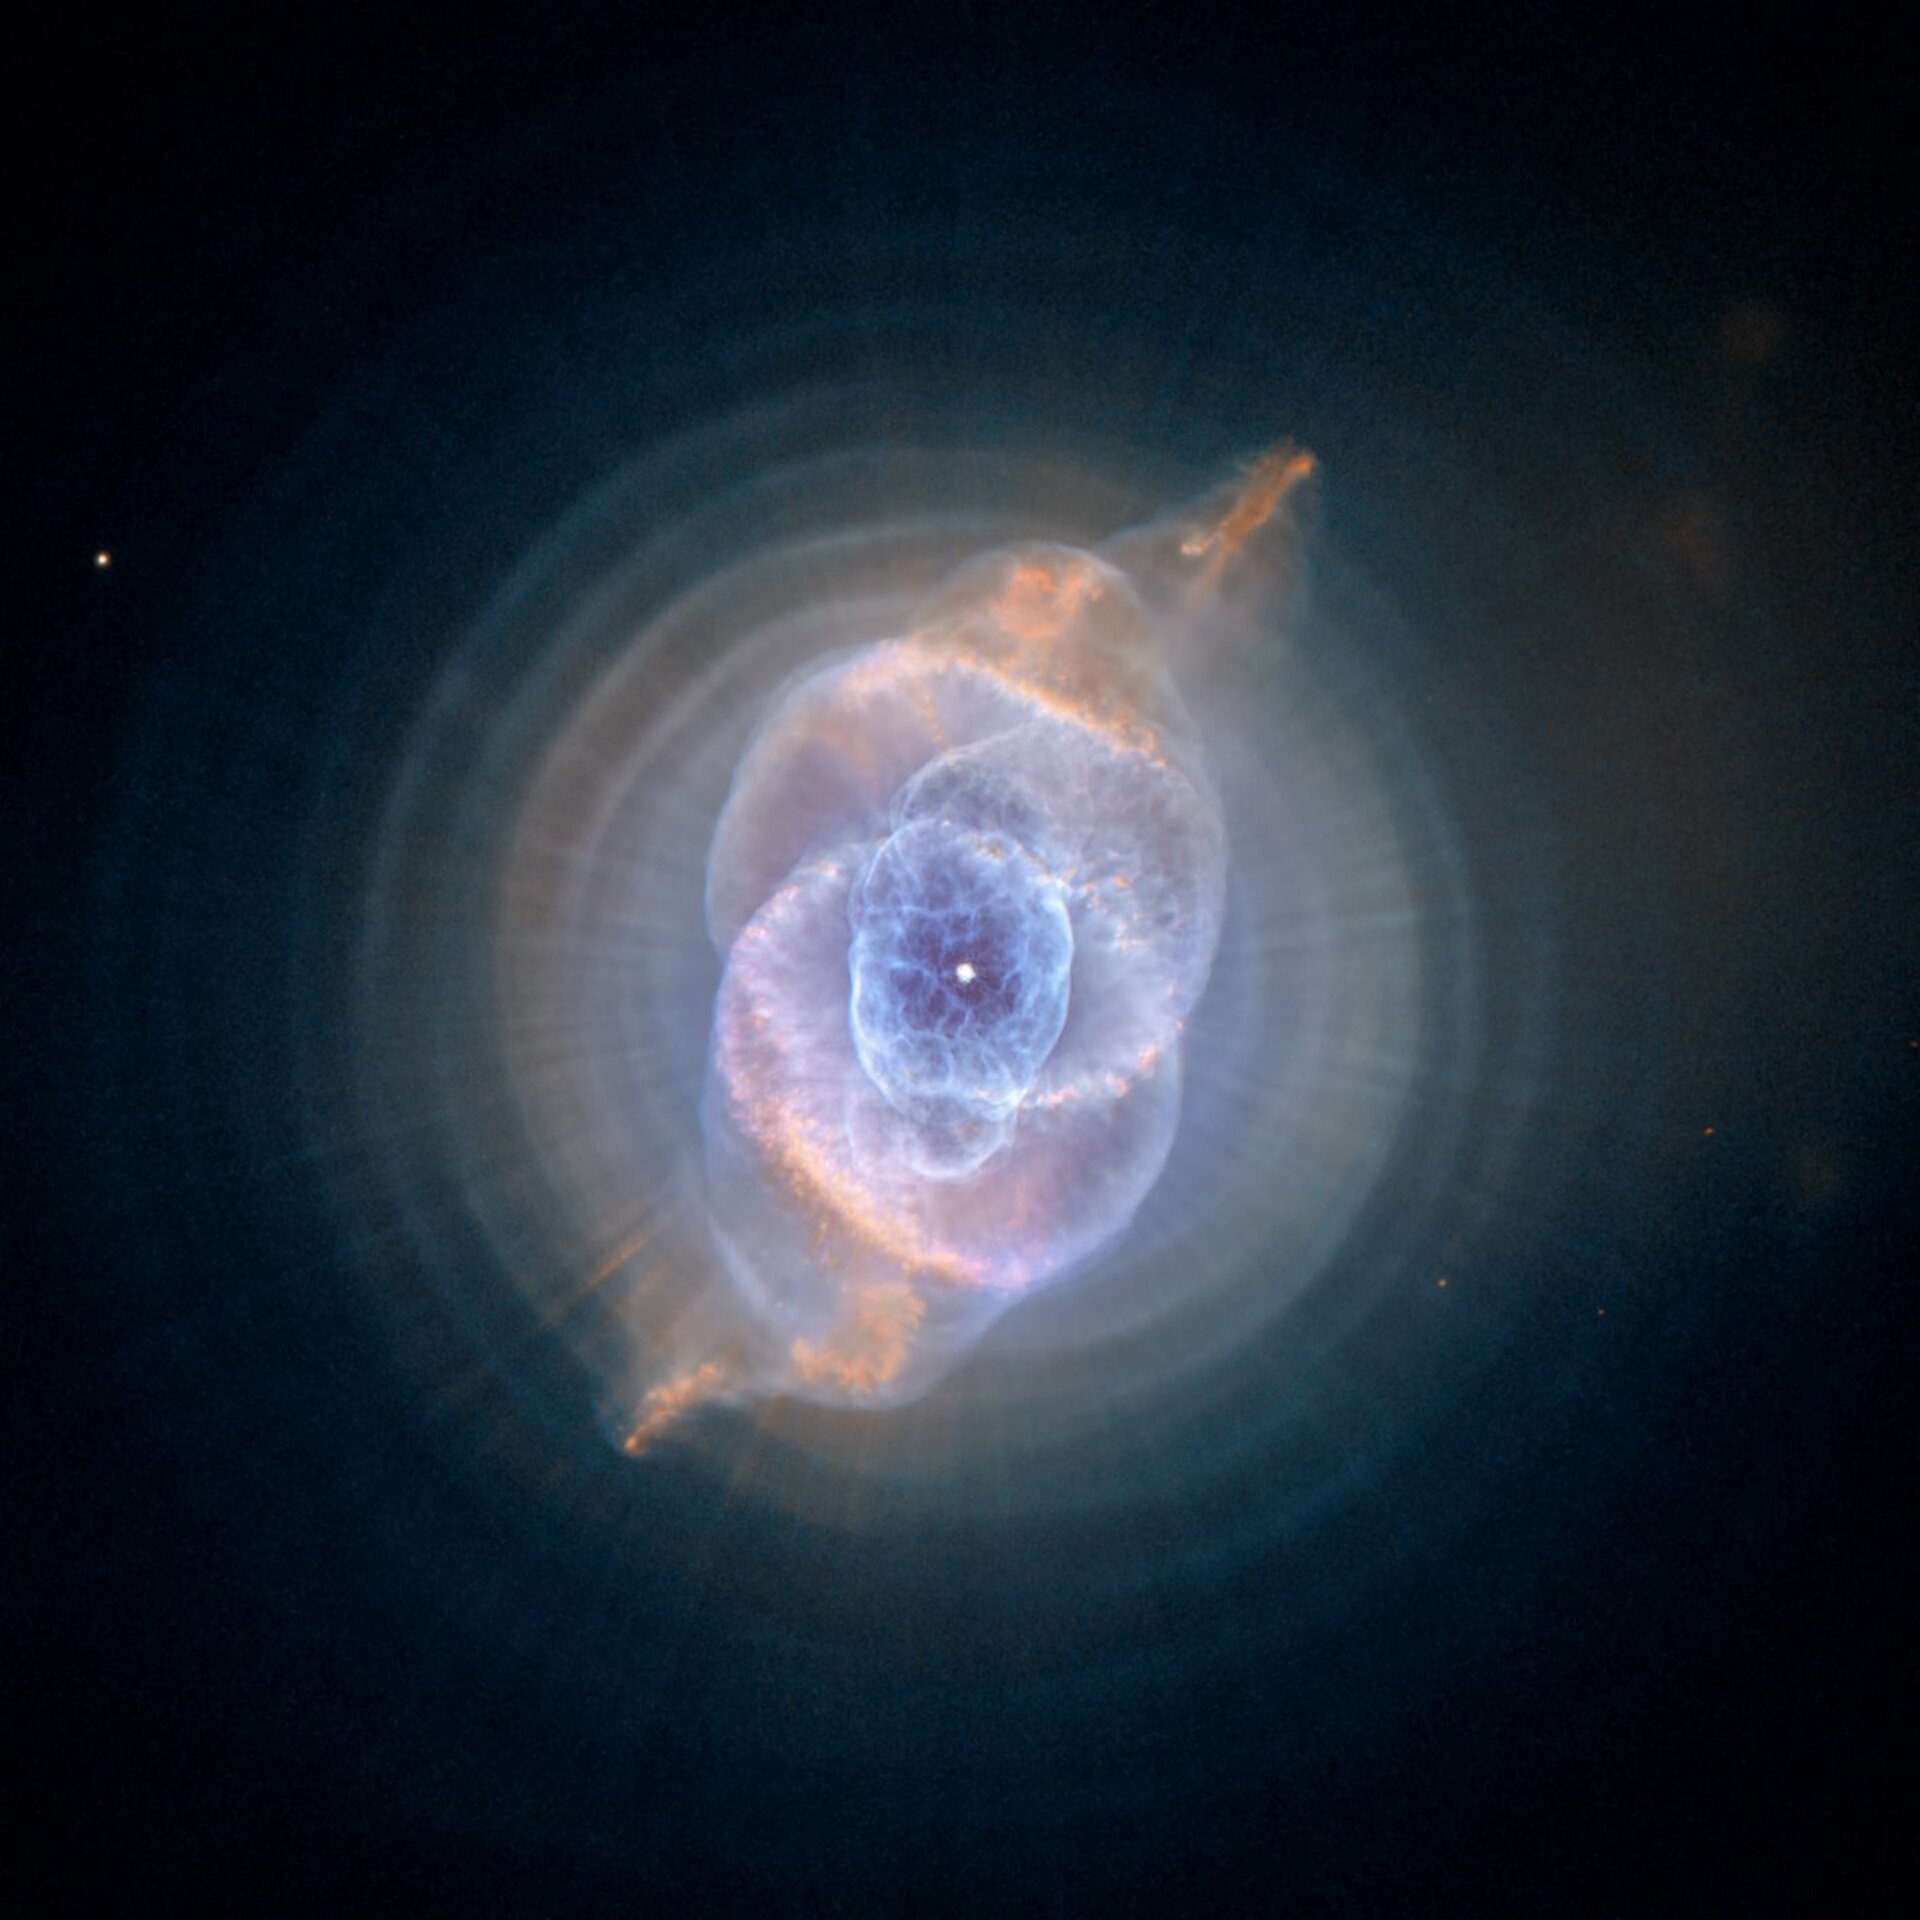
\includegraphics[width=0.7\textwidth]{CatEye.jpg}
        \caption{La nebulosa Ojo de Gato (NGC 6543) fotografiada por el Telescopio Espacial Hubble. En su centro hay una joven estrella enana blanca ubicada a 11.000 años luz de la Tierra.}
        \label{CatEye}
    \end{figure}



La luminosidad, $L$, de la enana blanca sol se ha modelado matemáticamente como una función del tiempo, $t$, dando

$$y = \text{Log}_{10}L(t) \quad \text{y} \quad x = \text{Log}_{10}t$$

donde $t$ está en unidades de años y $L$ en múltiplos de la potencia solar actual ($3.8 \times 10^{26}\W$). El dominio de la función es $[+3.8, +10.5]$.

$$y(x) = 0.0026x^5 - 0.1075x^4 + 1.6895x^3 - 12.742x^2 + 45.396x - 59.024$$
\begin{itemize}

	\item El dominio sobre el cual $y(x)$ se aplica como una aproximación está dado por el intervalo logarítmico $[+3.8, +10.4]$. ¿A qué lapso de años corresponde esto?

	\item Graficar $y(x)$ sobre el dominio establecido usando una calculadora gráfica.

	\item ¿Para qué valores de $t$ en años se cumple que $y=0$, y cómo se interpreta esto físicamente en términos de $L$ y $t$? 
\end{itemize}

\end{problema}

\newpage

\begin{problema}
La búsqueda de una importante partícula teórica llamada Bosón de Higgs está en marcha en el Gran Colisionador de Hadrones, que comenzó a operar el 23 de noviembre de 2009. 

    \begin{figure}[H]
        \centering
        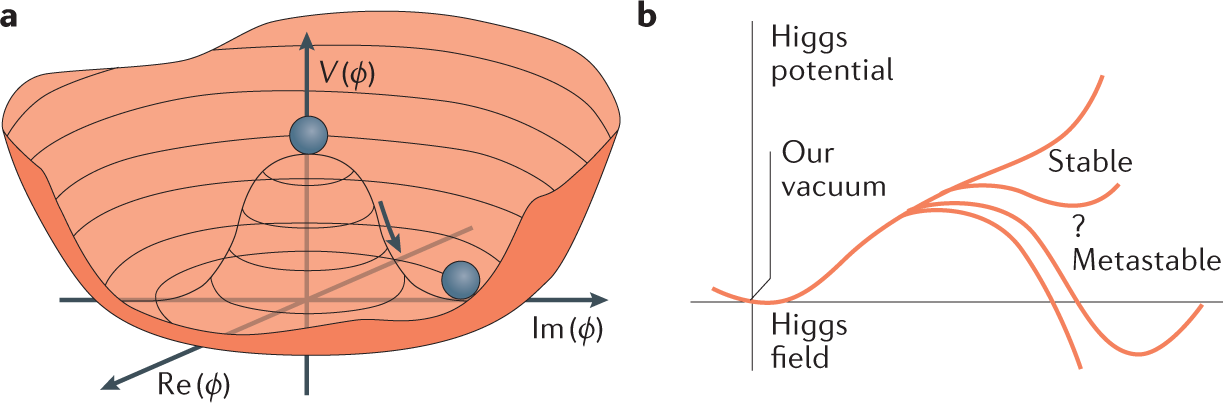
\includegraphics[width=0.7\textwidth]{Higgs.png}
        \caption{Representación esquemática del potencial del campo de Higgs}
        \label{Higgs}
    \end{figure}

La masa del Bosón de Higgs en realidad no es constante, sino que depende de la cantidad de energía que se utiliza para crearlo. Este comportamiento notable puede describirse mediante las propiedades de la siguiente ecuación:

$$V(x) = 2x^4 - (1 - T^2)x^2 + \frac{1}{8}$$

Esta ecuación describe la energía potencial, $V$, almacenada en el campo que crea el Bosón de Higgs. La variable $x$ es la masa del Bosón de Higgs, y $T$ es la energía de colisión utilizada para crear esta partícula. El campo de Higgs representa una nueva fuerza 'hiperdébil' en la Naturaleza que es más fuerte que la gravedad, pero más débil que la fuerza electromagnética. El Bosón de Higgs es la partícula que transmite el campo de Higgs, así como el fotón es la partícula que transmite el campo electromagnético.
\begin{enumerate}
\item Usando una calculadora gráfica, ¿cuál es la forma de la función $V(x)$ sobre el dominio $[0, +1]$ para una energía de colisión de: 
	\begin{enumerate}
		\item $T=0$? 
		\item $T=0.5$? 
		\item $T = 0.8$ 
		\item $T=1.0$
	\end{enumerate}
	\item La masa del Bosón de Higgs se define por la ubicación del mínimo de $V(x)$ sobre el dominio $[0, +1]$. Si la masa, $M$ en $\GeV$, del Bosón de Higgs se define como $M = 300x$, ¿cómo cambia la masa predicha del Bosón de Higgs a medida que el valor de $T$ aumenta de $0$ a $1$?
\end{enumerate}
\end{problema}

\begin{problema}

Un concepto importante en cosmología es que el 'espacio vacío' entre estrellas y galaxias ¡en realidad no está vacío en absoluto! Hoy, la cantidad de energía invisible oculta en el espacio es suficiente para ser detectada como Energía Oscura, a medida que los astrónomos miden la velocidad de expansión del universo. Poco después del Big Bang, esta Energía Oscura causó que el universo se expandiera enormemente en menos de un segundo. Los cosmólogos llaman a este periodo temprano de la era del Big Bang, Inflación Cósmica.

    \begin{figure}[H]
        \centering
        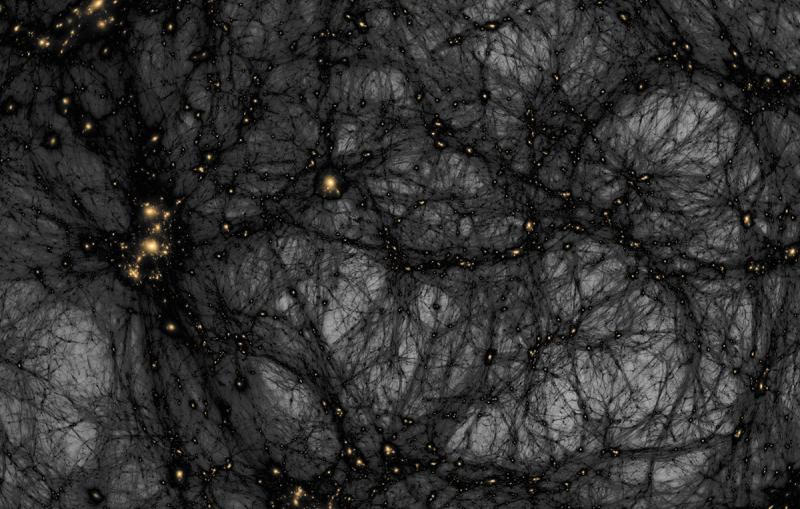
\includegraphics[width=0.7\textwidth]{DarkMatter.jpg}
        \caption{Ilustación de la materia oscura}
        \label{DarkMatter}
    \end{figure}


Una propiedad interesante de este nuevo campo de 'energía oscura', cuya energía está representada por la función $V(x)$, es que la forma de esta función cambia a medida que la temperatura del universo cambia. El resultado es que la forma en que este campo, representado por la variable $x$, interactúa con las otras partículas elementales en la naturaleza, cambia. A medida que ocurre este cambio de temperaturas muy altas ($T=1$) a temperaturas muy bajas ($T=0$), ¡el universo experimenta la Inflación Cósmica!

$$V(x) = 2x^4 - (1-T^2)x^2 + \frac{1}{8}$$

\begin{enumerate}
	\item ¿Cuál es el dominio y rango de la función $V(x)$?

	\item ¿Cuál es el eje de simetría de $V(x)$?

	\item ¿Es $V(x)$ una función par o impar?

	\item  Para $T=0$, ¿cuáles son los puntos críticos de la función en el dominio $[-2, +2]$?

	\item En el dominio $[0, +2]$, ¿dónde se ubican los mínimos y máximos locales para $T=0$?

	\item Usando una calculadora gráfica , grafica $V(x)$ para los valores $T=0, 0.5, 0.8$ y $1.0$ en el dominio $[0, +1]$. 
	Tabula el valor de x del mínimo local como una función de $T$. 
	En términos de su ubicación en x, ¿qué crees que le sucede al comportamiento final del mínimo de $V(x)$ en este dominio a medida que $T$ aumenta?

	\item ¿Cuál es la diferencia de energía del vacío $V = V(0) - V(1/2)$ durante la Era de la Inflación Cósmica?

	\item La energía real almacenada en el 'espacio vacío' dada por $V(x)$ tiene unidades físicas de densidad de energía en múltiplos de $10^{35}\J/\m^3$. ¿Cuál es la densidad de energía disponible durante la Era de la Inflación Cósmica en estas unidades físicas?
\end{enumerate}

\end{problema}


\cite{algebra2}
\bibliographystyle{plainurl}
\bibliography{bibliografia} % Nombre del .bib

\end{document}
